\chapter{以LED與PD建立三維相對位置之演算法}
\label{chp:3}

如\ref{chp:LEDPD_problem}章所述,現今LED與PD的定位方法雖具有靈活應用的潛力,然而在單點對單點的定位中,仍未有可以進行三維定位,且不限制目標平面與量測平面平行的方法。因此,本章節將提出一定位演算法,利用$L\times P$個LED對PD的電流大小資訊,計算出三維相對定位,且不需限制目標平面與使用者平面平行,並在模型中將LED與PD的朗博次方考慮進去。

\begin{figure}[h!]
    \centering
    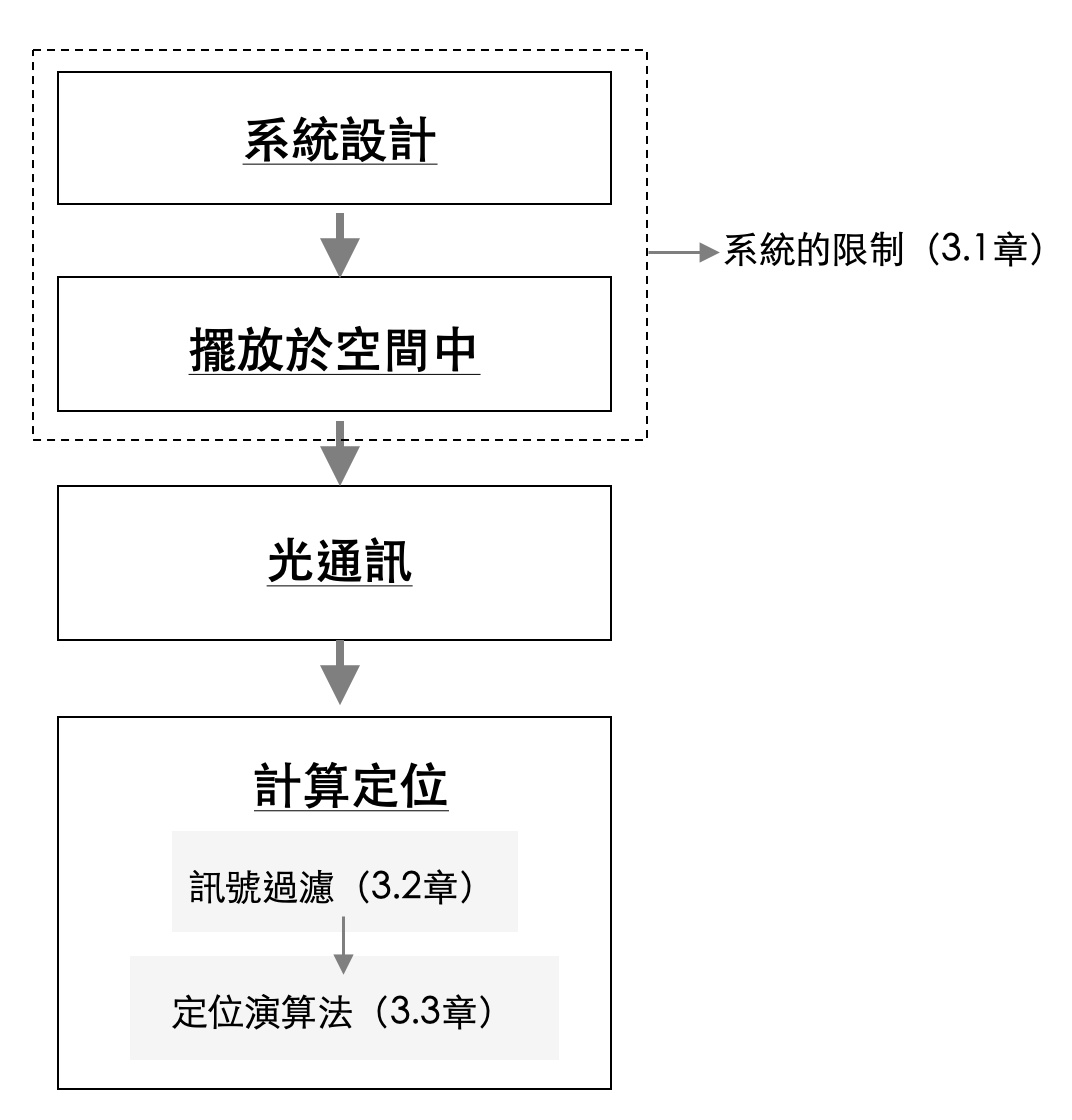
\includegraphics[width=9cm]{ch3pic/chp3_flow.png}
    \caption{第三章章節與定位流程對應}
    \label{pic:chp3_flow}
\end{figure}


本章節的論述順序可以參考圖\ref{pic:chp3_flow},根據LED與PD定位系統流程圖(圖\ref{pic:lp_system_flow})重新整理,著重在計算定位的方法上。首先,\ref{chp:algorithm_constraint}章定義本方法對系統設計的拘束條件,再於\ref{chp:algorithm_filter}章中針對電流資訊進行過濾,於\ref{chp:algorithm}章中解釋如何由過濾過的訊號,計算出三維相對定位,最後於\ref{chp:algorithm_ad_dis}章中整理此演算法的優缺點。








\section{系統的限制}
\label{chp:algorithm_constraint}

根據\ref{chp:LEDPD_problem}章中的論述,我們知道現今文獻上需要透過對系統限制,以將光傳遞模型進行簡化,來求解相對位置。本段落將條列式列出本研究的定位演算法中,使用的系統限制:

    \begin{description}

        \item[1. 硬體選用限制:]系統使用的LED皆為同款式,PD亦然。
        \item[2. PD擺放位置限制:]PD擺放位置相同並於PD座標系原點,$^P\boldsymbol{P}_p=
        \left[\begin{array}{ccc}0&0&0\end{array}\right]^T$
        \item[3. LED擺放位置限制:]LED擺放位置相同並於LED座標系原點,$^L\boldsymbol{P}_l=
        \left[\begin{array}{ccc}0&0&0\end{array}\right]^T$

    \end{description}
   
    \begin{figure}[h!]
        \centering
        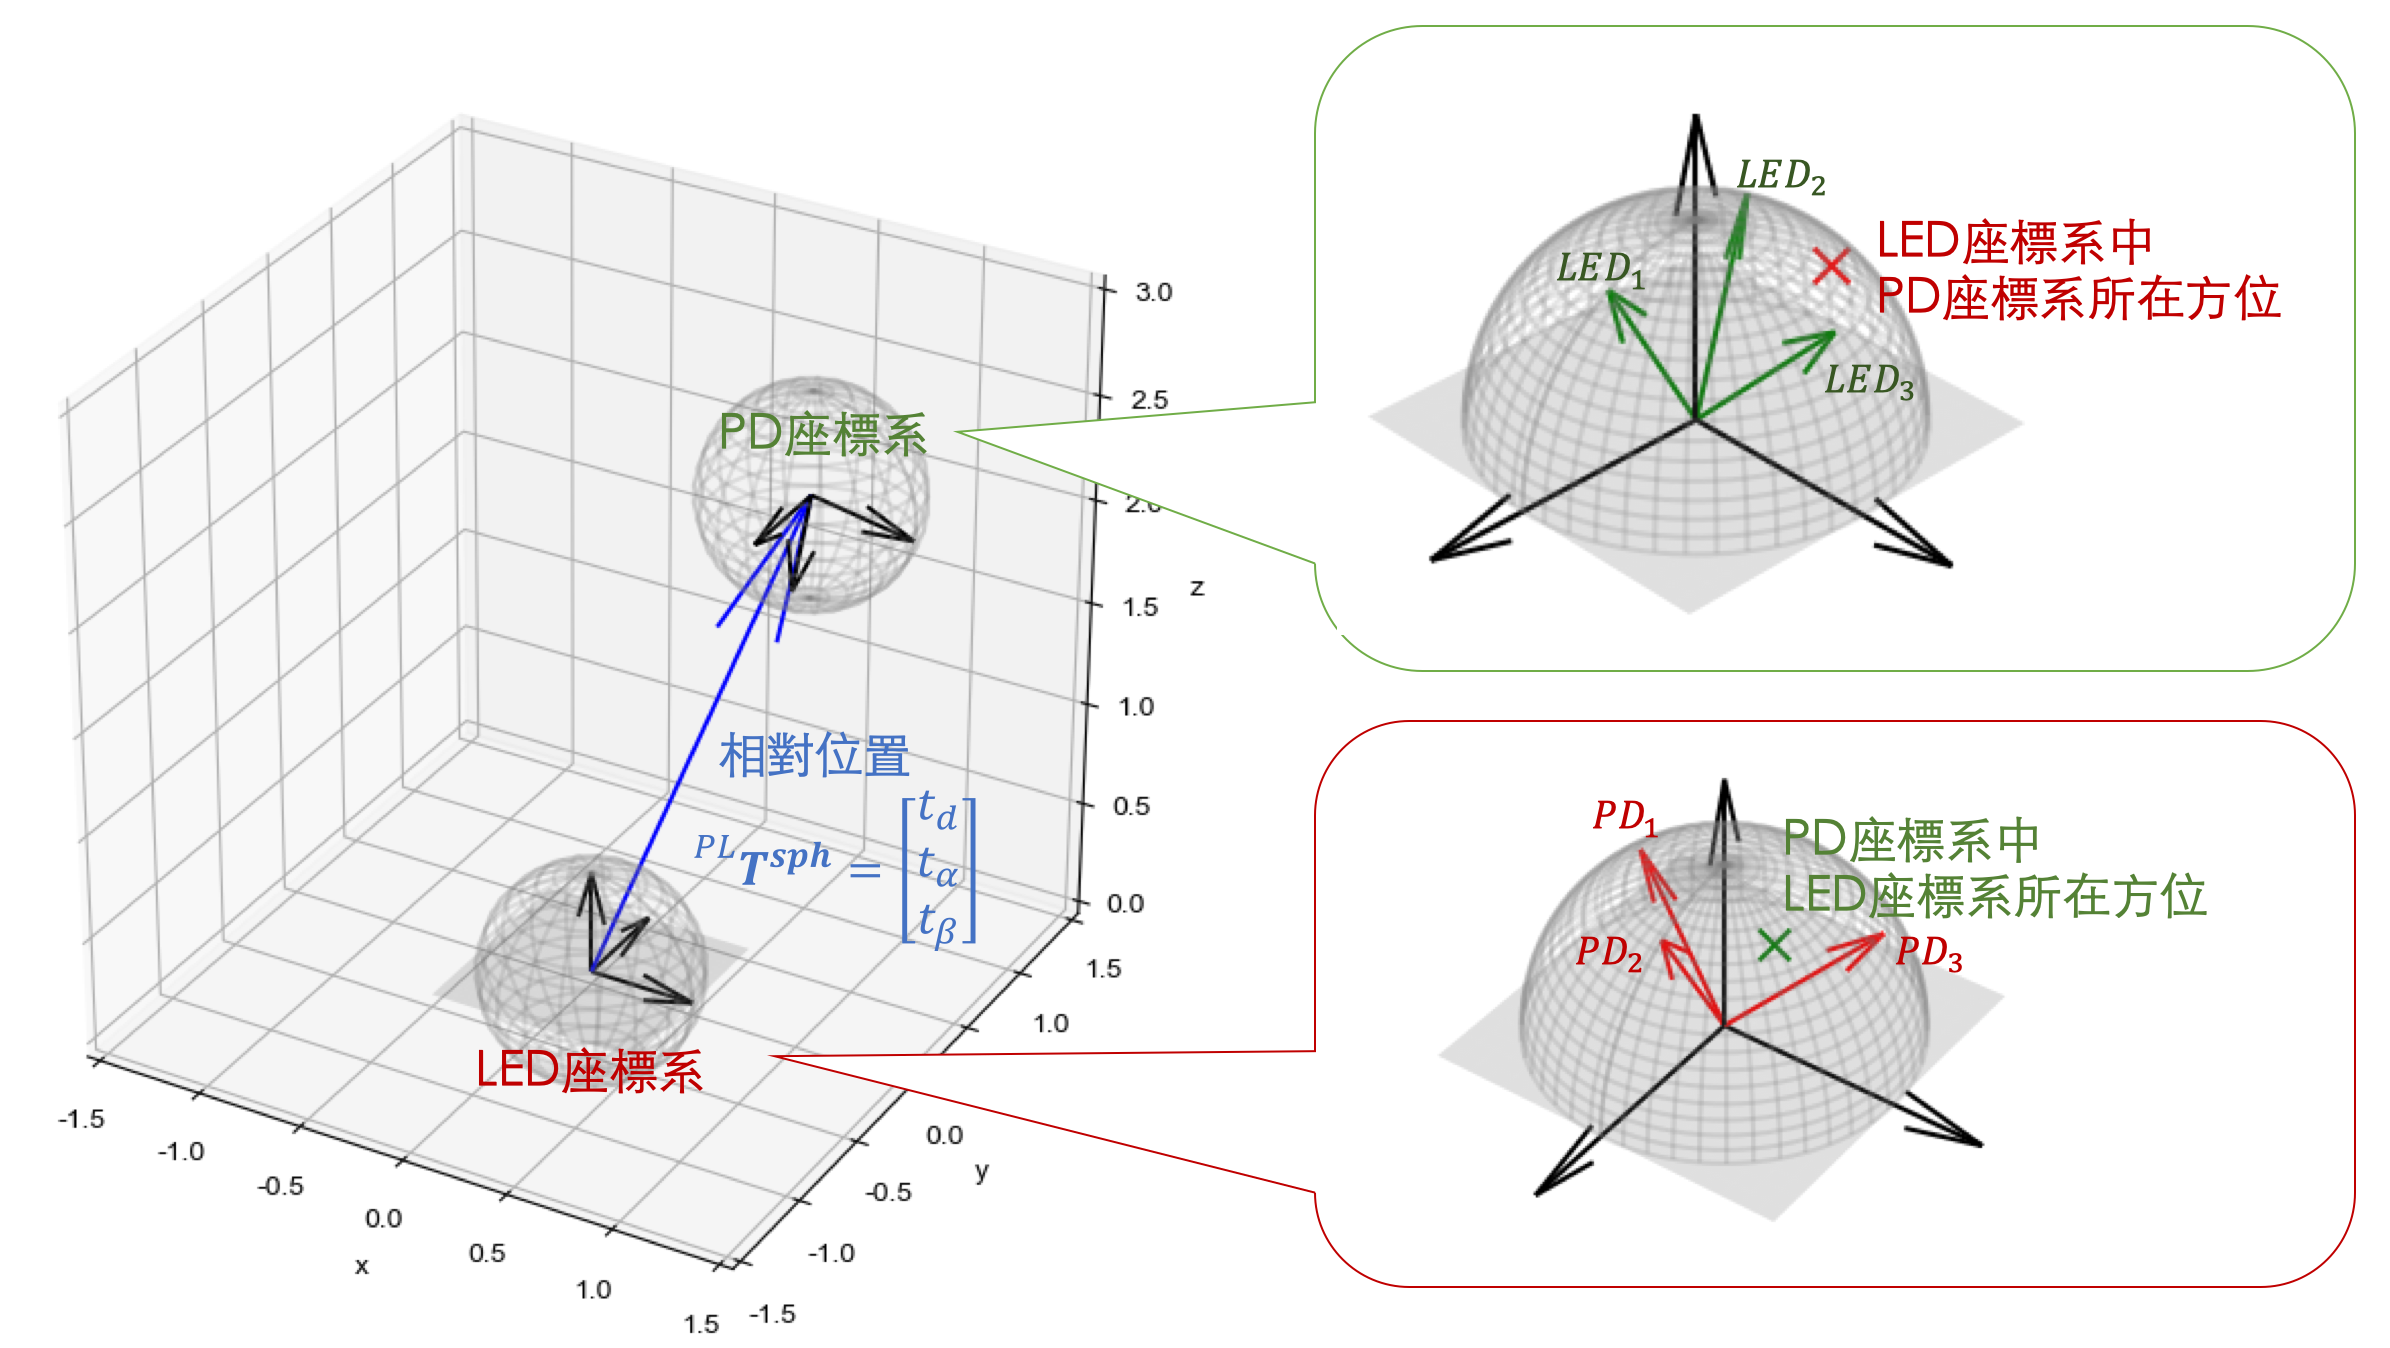
\includegraphics[width=14cm]{ch3pic/algorithm_place.png}
        \caption{PD與LED組態皆限制擺放於原點的系統組態}
        \label{pic:algorithm_coor}
    \end{figure}

    根據以上限制,LED與PD的定位系統可以呈現於圖\ref{pic:algorithm_coor},LED與PD座標系中的硬體皆固定於各自的座標系原點,指向則並無特別限制。在將LED與PD組態設計完成後,座標系放置於空間中兩個點進行定位,其中,各LED到各PD的距離$D_{lp}$皆相同,都是兩座標系之間的距離$t_d$,我們便將光傳遞模型\ref{eqn:model}簡化為\ref{eqn:model_algorithm}。

    \begin{equation}
        \label{eqn:model_algorithm}
        Ie_{lp} = \begin{cases}Re\frac{PtA(Ml+1)}{2\pi}\frac{\cos\phi_{lp}^{Mp}\cos \theta_{lp}^{Ml}}{D^2} , & \text { if } Ie_{lp}<s \\ s, & \text { otherwise }\end{cases}
    \end{equation}

    然而,大多文獻在討輪三維定位時是以卡氏座標系定義相對位置$^{PL}\boldsymbol{T}=\left[\begin{array}{ccc}t_x&t_y&t_z\end{array}\right]^T$,而我們提出的演算法則是以球座標系定義$^{PL}\boldsymbol{T}^{sph}=\left[\begin{array}{ccc}t_d&t_{\alpha}&t_{\beta}\end{array}\right]^T$,因此我們需求出的三個未知數為$t_d,t_\alpha,t_\beta$三項,$t_d$即為兩座標系之間的距離,而$t_{\alpha},t_{\beta}$則為LED座標系所在「方位」。


\section{訊號過濾}
\label{chp:algorithm_filter}

由於PD電流會飽和的特性,已飽和的電流與距離與出入射角無關了,無法用來獲得相對定位,因此我們需將已飽和的電流$Ie_{lp}>s$訊號忽略。除此之外,過小的電流也有可能為雜訊,因此也需設定一閥值$Th$,將小於閥值的電流訊號也忽略,剩餘的訊號則為可運用於計算三維定位的資訊。在訊號過濾後,第$l$個LED中還剩下$Fp_l$個PD電流數值可使用,而第$p$個PD中則剩下$Fl_p$個LED對應的電流數值可使用,參考圖\ref{pic:after_filter}。

\begin{figure}[h!]
    \centering
    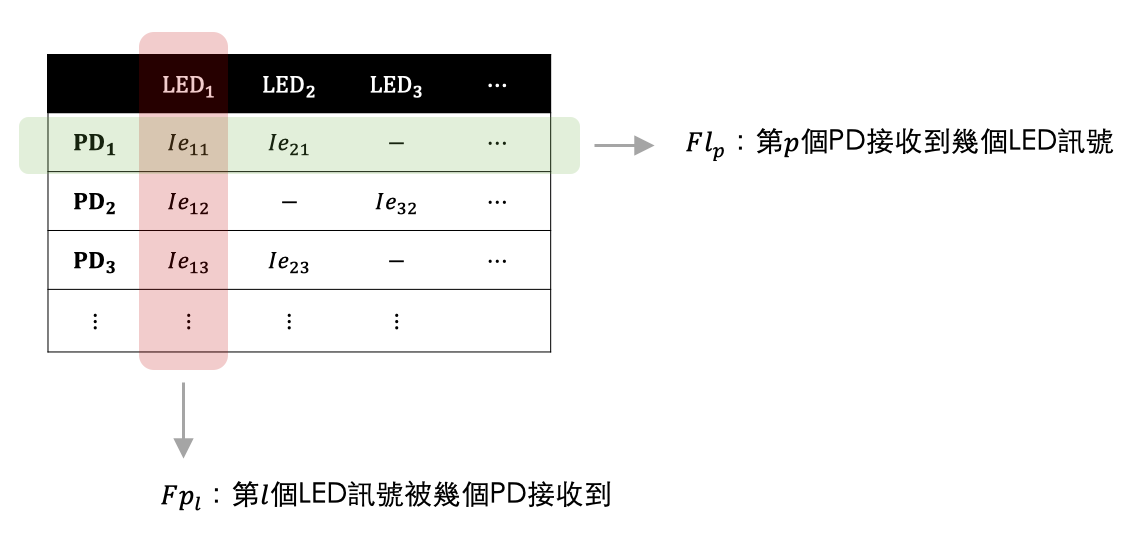
\includegraphics[width=15cm]{ch3pic/after_filter.png}
    \caption{訊號過濾後各LED與各PD所剩的訊號數量示意圖}
    \label{pic:after_filter}
\end{figure}

\section{定位演算法}
\label{chp:algorithm}

\begin{figure}[h!]
    \centering
    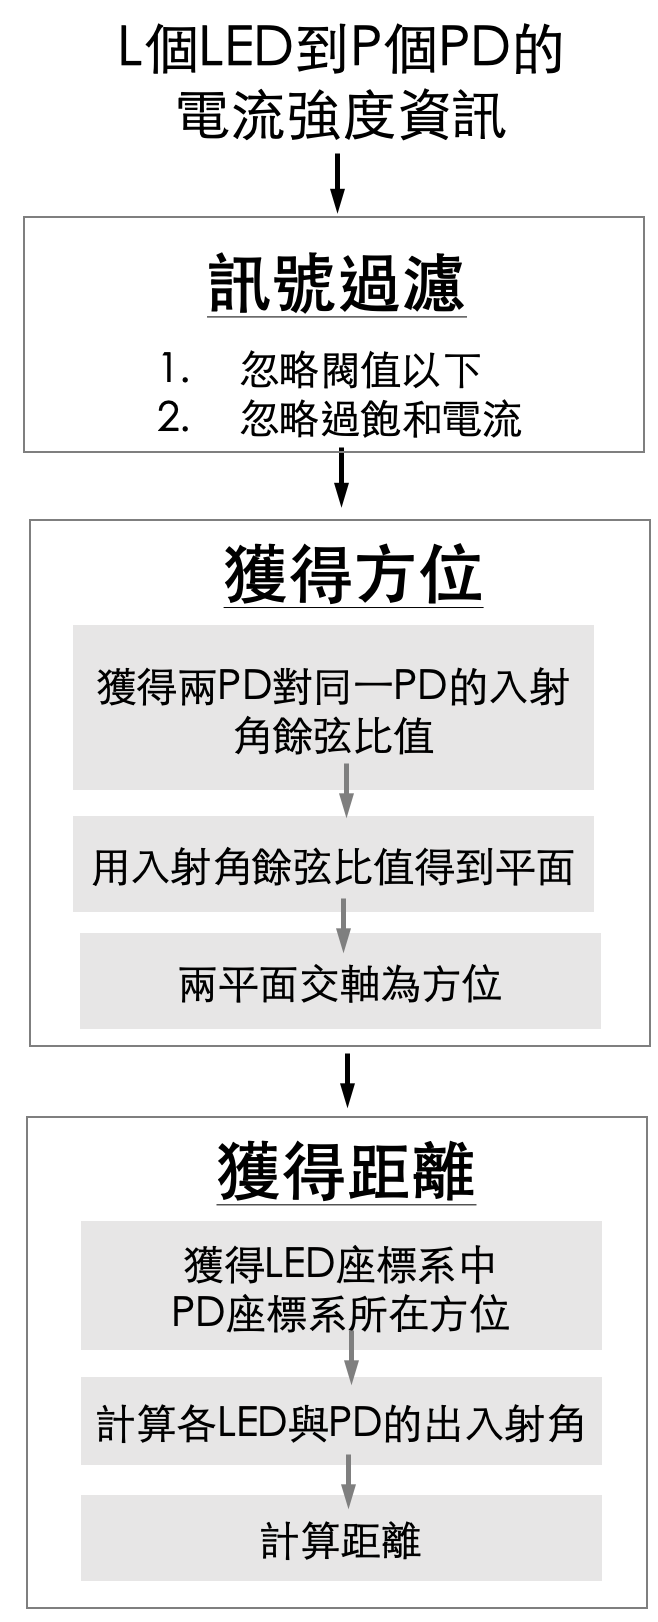
\includegraphics[width=6cm]{ch3pic/algorithm_flow.png}
    \caption{本研究所提出的定位演算法流程}
    \label{pic:algorithm_flow}
\end{figure}

本章結提出的定位演算法,為LED與PD系統流程圖\ref{pic:chp3_flow}中的定位演算法步驟,定位演算法的步驟則呈現於圖\ref{pic:algorithm_flow},依序從\ref{chp:solve_phi}章解出PD座標系中,LED座標系所在方位;\ref{chp:solve_D}綜合LED與PD方位資訊,解出距離。

為了方便表示,將方位以符號表示$^{PL}\boldsymbol{Tv}^{sph} = \left[\begin{array}{ccc}1&t_{\alpha}&t_{\beta}\end{array}\right]^T$,方位為單位向量,可用單位圓表示方位的可行解範圍。





    \subsection{求解方位}
    \label{chp:solve_phi}

    首先,過濾後的訊號即不需考慮過飽和的狀況,因此式\ref{eqn:model_algorithm}可改寫為式\ref{eqn:model_algorithm_filter}。

    \begin{equation}
        \label{eqn:model_algorithm_filter}
        \begin{aligned}
            Ie_{lp}(D_{lp},\theta_{lp},\phi_{lp}) &= Re\frac{PtA(Ml+1)}{2\pi}\frac{{\cos\phi}^{Mp}{\cos\theta}^{Ml}}{D^2}\\
            & = Re\frac{PtA(Ml+1)}{2\pi}\frac{{(^{P}\boldsymbol{V}_p\cdot\boldsymbol{D})}^{Mp}{(-^{PL}\boldsymbol{V}_l\cdot\boldsymbol{D})}^{Ml}}{D^4}
        \end{aligned}
    \end{equation}

    解方位的流程詳細如圖\ref{pic:orient_flow},於\ref{chp:cosine_ratio}章到\ref{chp:orient_average}章詳細介紹取得方位$^{PL}\boldsymbol{Tv}^{sph} = \left[\begin{array}{ccc}1&t_{\alpha}&t_{\beta}\end{array}\right]^T$的過程。

    \begin{figure}[h!]
        \centering
        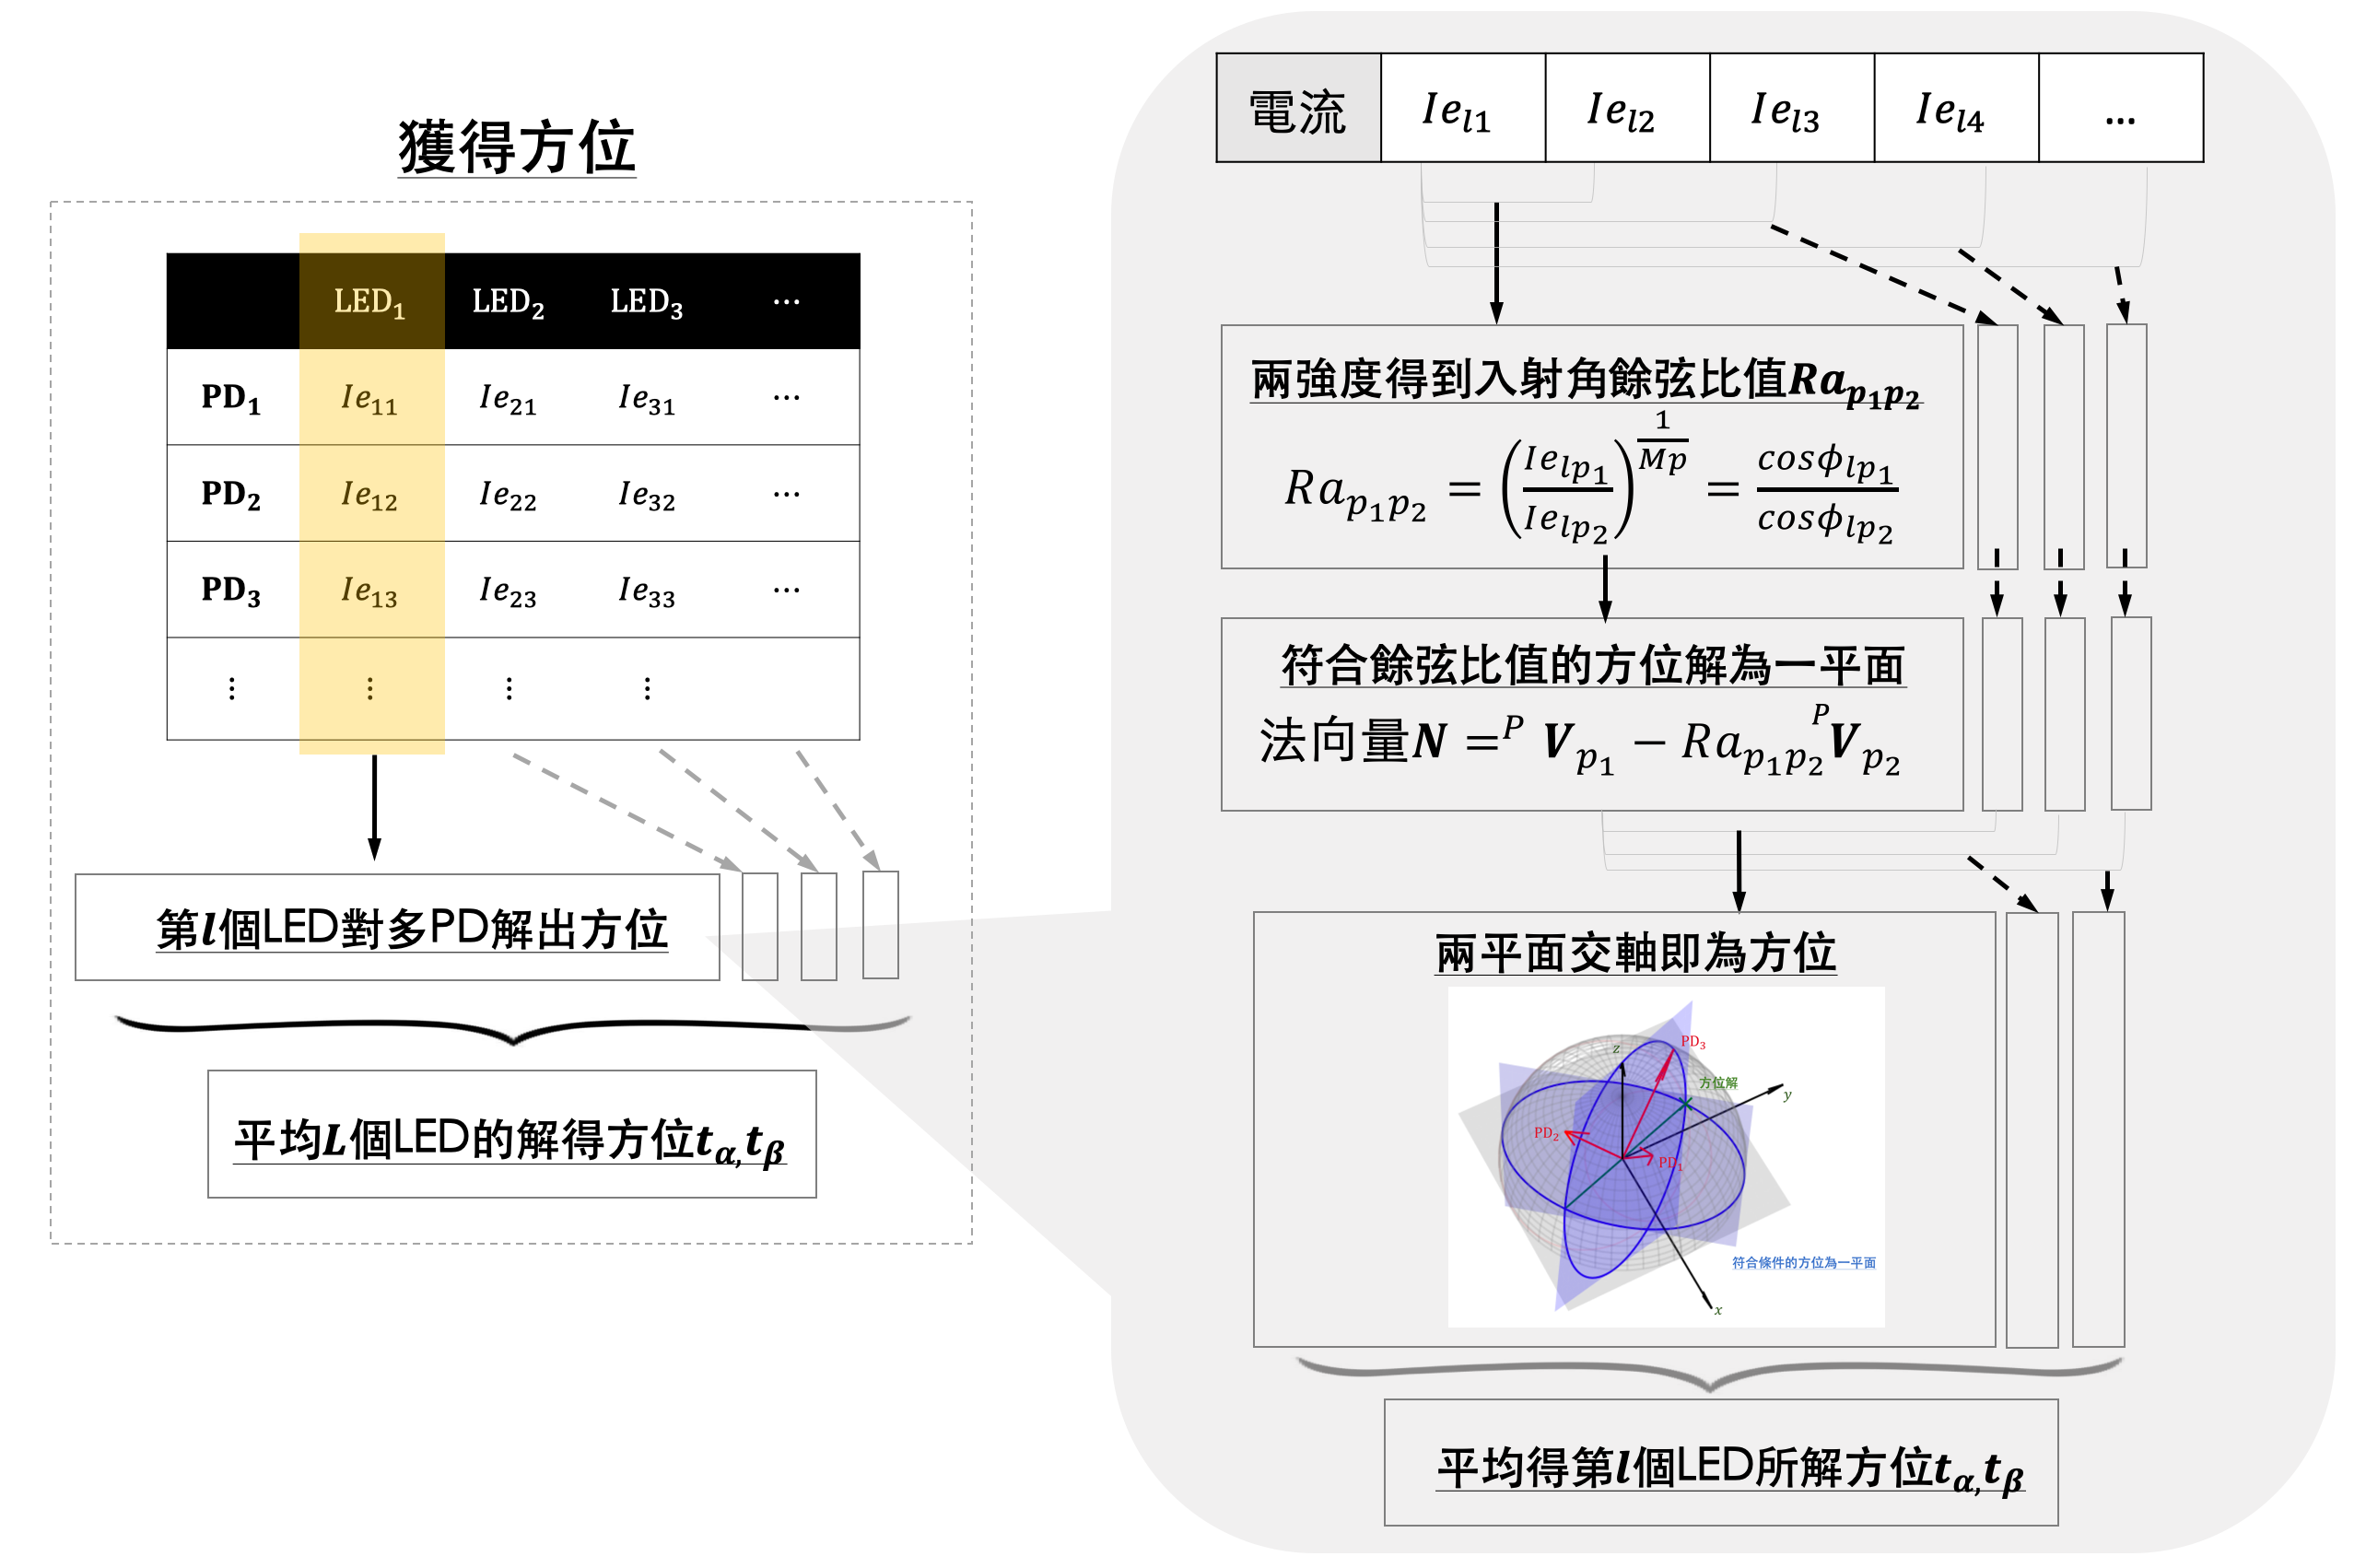
\includegraphics[width=14cm]{ch3pic/orient_flow.png}
        \caption{本研究定位演算法中解方位的流程}
        \label{pic:orient_flow}
    \end{figure}

    \subsubsection{獲得兩PD對同一LED的入射角餘弦比值}
    \label{chp:cosine_ratio}

        \begin{figure}[h!]
            \centering
            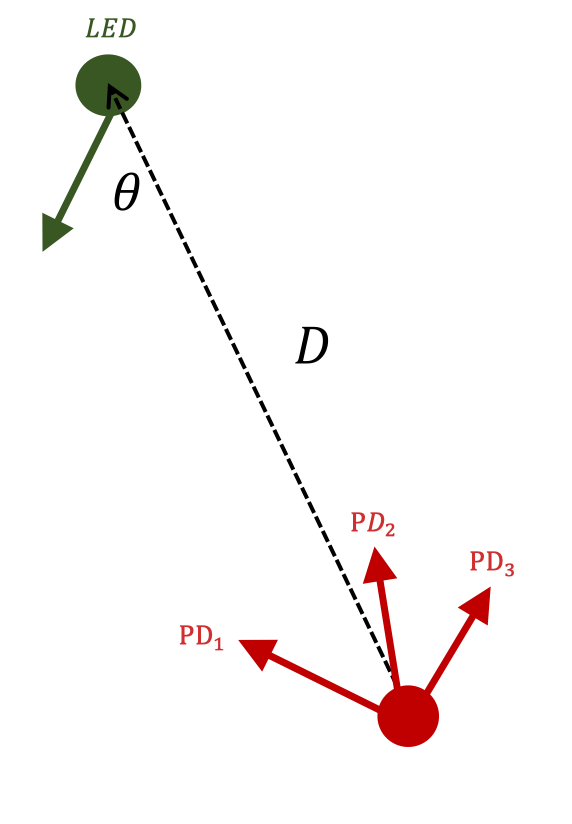
\includegraphics[width=5cm]{ch3pic/1led_mulpd.png}
            \caption{同一LED與多個PD之間的幾何關係}
            \label{pic:1led_mulpd}
        \end{figure}

        當我們僅考慮第$l$個LED的資訊時,如圖\ref{pic:1led_mulpd}所示,各PD與該LED之間的LED出射角$\theta_{lp}$以及距離$D_{lp}$都一樣;因此,式\ref{eqn:model_algorithm_filter}中的三個變數只剩下PD入射角$\phi_{lp}$,而我們於式\ref{eqn:cosine_ratio}中,將不同PD對同樣第$l$個LED的強度訊號相除,可得到入射角餘弦比值的朗博次方。藉由將其開朗博次方根,我們得到編號$p_1$與$p_2$的PD,對第$l$個LED入射角餘弦比值$Ra_{p_1p_2}$。
    
        \begin{equation}
            \label{eqn:cosine_ratio}
            \begin{aligned}
                \frac{Ie_{lp_1}}{Ie_{lp_2}}={(\frac{\cos\phi_{lp_1}} {\cos\phi_{lp_2}})}^{Mp}\\
                Ra_{p_1p_2} = {( \frac{Ie_{lp_1}}{Ie_{lp_2}})} ^{\frac{1}{Mp}} = \frac{\cos\phi_{lp_1}}{\cos\phi_{lp_2}}
            \end{aligned}
        \end{equation}

        兩個PD比較即可得到一個入射角比值,而為了更有系統性的進行兩兩比較,我們選擇一參考PD,其餘PD訊號都與參考PD做比較,即可有效率的完成動作。其中,對第$l$個LED來說,過濾過後的訊號有$Fp_l$個,我們選擇第$r_c$個PD當作參考值,將其作為分母,其他PD電流值與其相比,總共得到$Fp_l-1$個比值$Ra_{pr_c}$

    \subsubsection{滿足入射角餘弦比值的方位解位於一通過原點之平面}
    \label{chp:solve_surface}
        
        於式\ref{eqn:cosine_ratio}中得到兩入射角餘弦比值,而我們需要從餘弦比值中得到方位關係,雖然兩角度的餘弦比值並沒有單一解,但是滿足入射角餘弦比值$Ra_{pr_c}$的方位解$^{PL}\boldsymbol{Tv}$,僅有可能位於一通過原點之平面,以下進行推導。
        
        首先,將式\ref{eqn:cosine_ratio}中的PD入射角$\phi_{lp}$,改寫為PD指向$^P\boldsymbol{V}_p$與入射方位$^{PL}\boldsymbol{Tv}$的內積,如式\ref{eqn:phi2dot}。
     

        \begin{equation}
            \label{eqn:phi2dot}
            \begin{aligned}
                \because \cos\phi_{lp} = ^{PL}\boldsymbol{Tv}\cdot^P\boldsymbol{V}_p\\
                \therefore Ra_{p_1r_c}
                =\frac{^{PL}\boldsymbol{Tv}\cdot^P\boldsymbol{V}_{p_1}}{^{PL}\boldsymbol{Tv}\cdot^P\boldsymbol{V}_{r_c}}
            \end{aligned}
        \end{equation}
        % \begin{equation}

        而式\ref{eqn:phi2dot}中的向量都以卡氏座標系展開,經過移項整理呈現於式\ref{eqn:surface}。

            \begin{gather}
                 \label{eqn:surface}
                 ^{PL}\boldsymbol{Tv} \cdot(Ra_{p_1r_c} ^P\boldsymbol{V}_{r_c}-
                 ^P\boldsymbol{V}_{p_1})=0
            \end{gather}
        % \end{equation}

        式\ref{eqn:surface}中的方位$^{PL}\boldsymbol{Tv}$,於空間中為一通過原點的平面,參考圖\ref{pic:solve_surface},透過兩個PD強度比較,我們可以得到一個方位解的可能平面。
       

       \begin{figure}[h!]
        \centering
        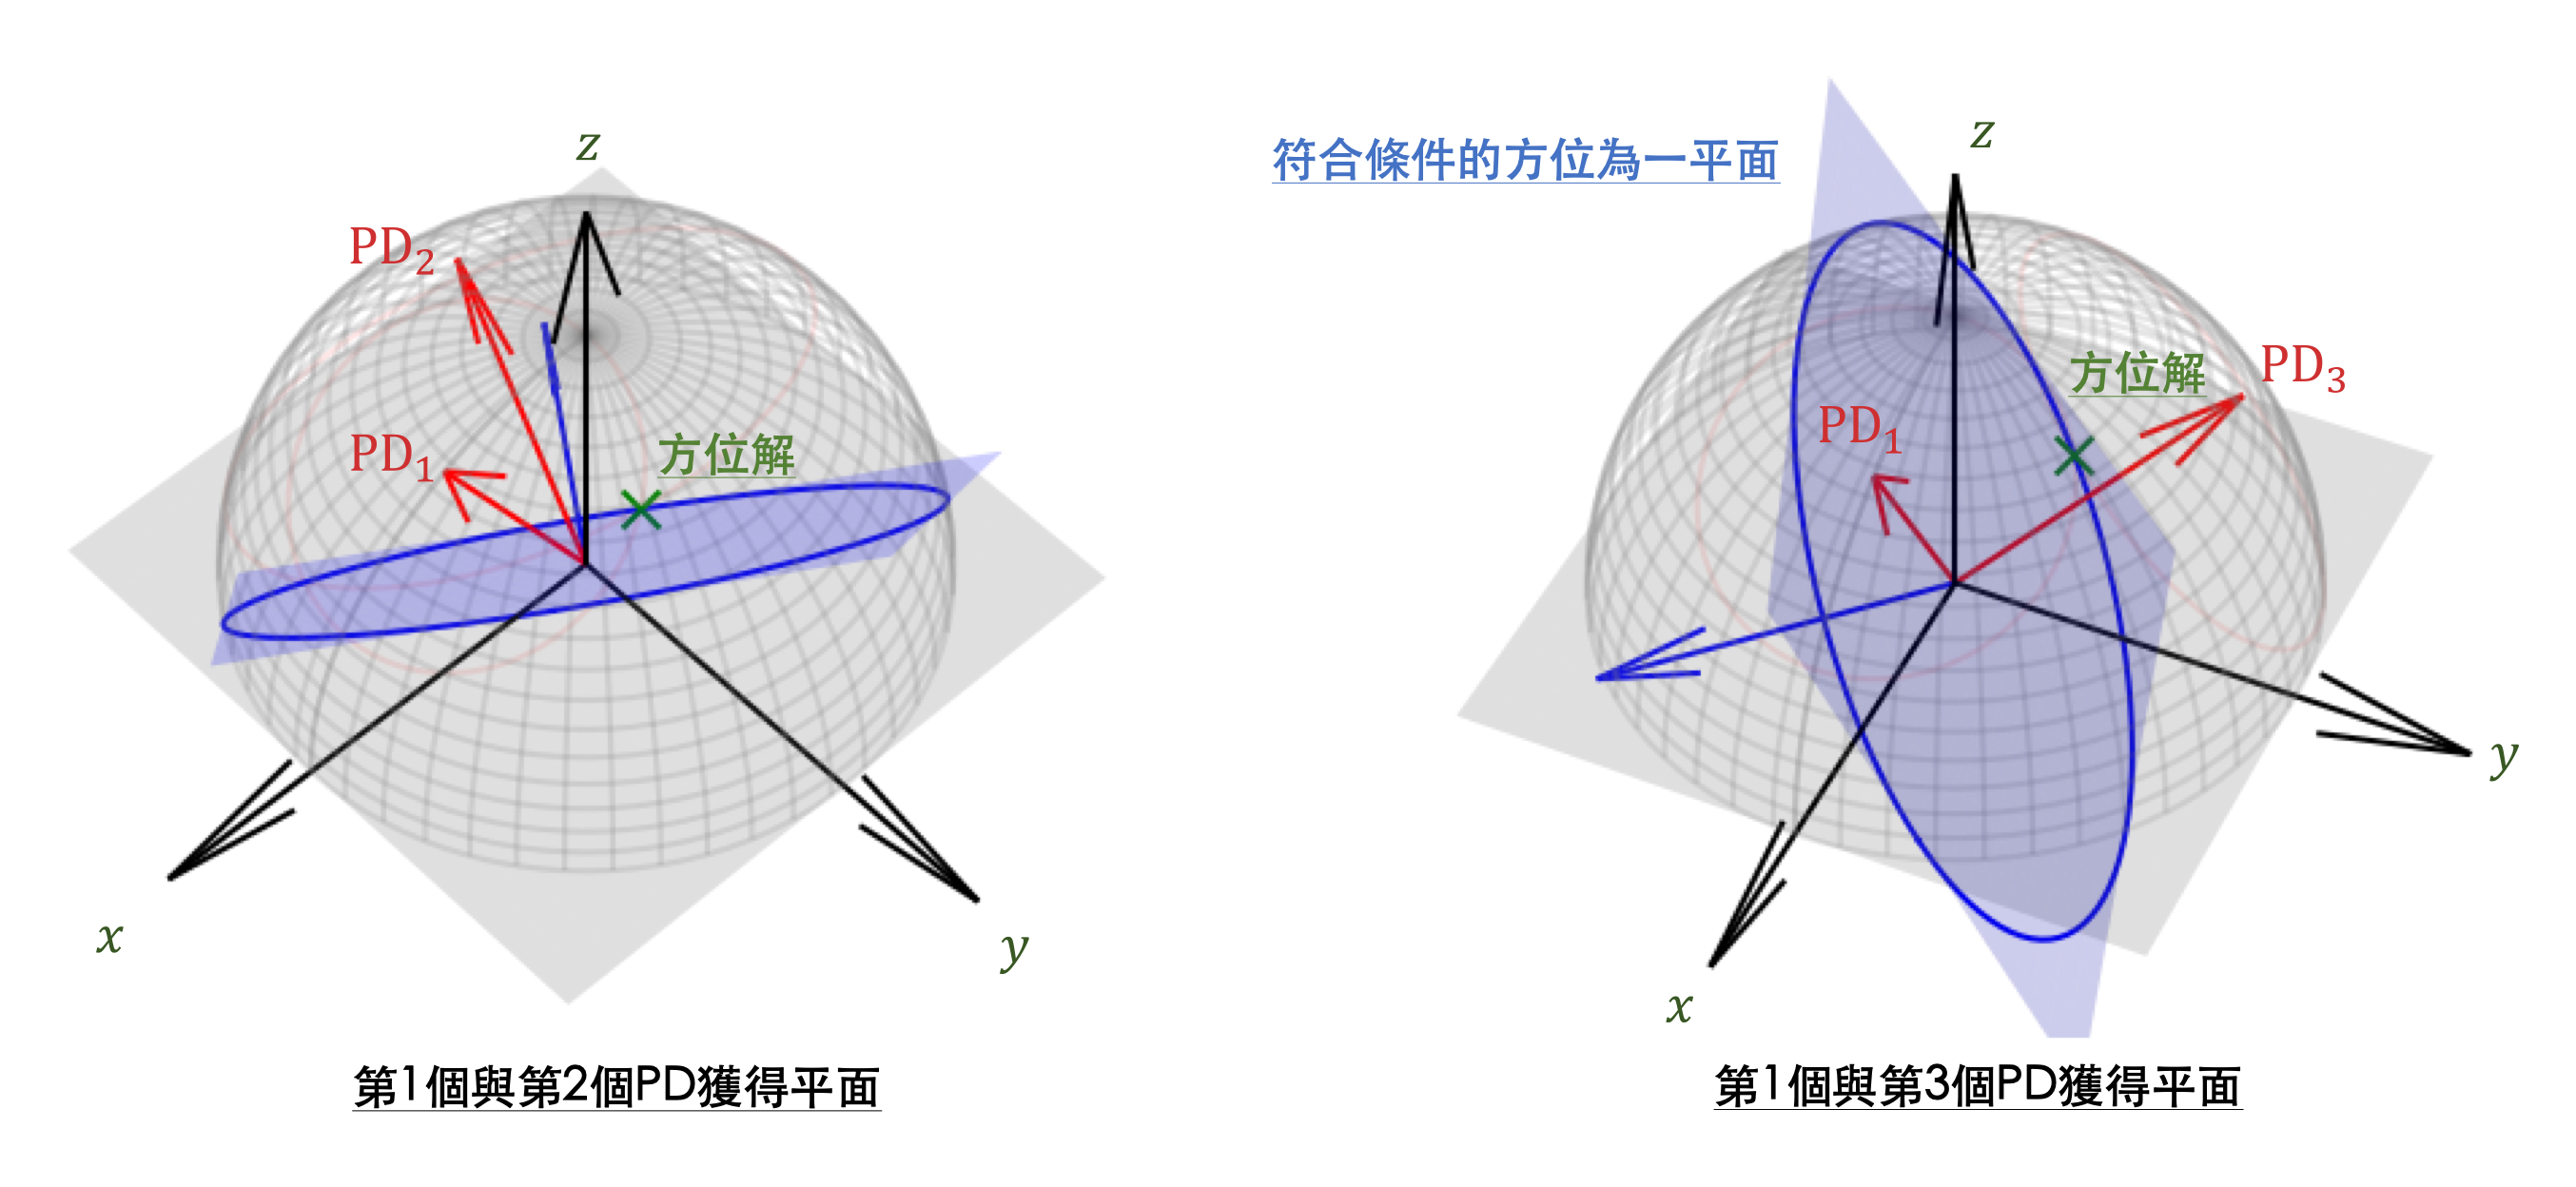
\includegraphics[width=14cm]{ch3pic/solve_surface.png}
        \caption{滿足入射角餘弦比值$Ra$的方位為通過原點之平面}
        \label{pic:solve_surface}
        \end{figure}

         
        我們將平面法向量以$\boldsymbol{N}_{p_1r_c}$表示於式\ref{eqn:surface_normal}中,小標$p_1,r_c$代表該平面是由第$p_1$個PD與第$r_c$個PD的入射角餘弦比值計算而得,其中$r_c$為作為參考值的PD編號。
        
        \begin{gather}
            \label{eqn:surface_normal}
            \boldsymbol{N}_{p_1r_c}  = {Ra_{p_1r_c}}{} ^P\boldsymbol{V}_{r_c}-
            ^P\boldsymbol{V}_{p_1}
       \end{gather}
        
        而於\ref{chp:cosine_ratio}章中,我們知道對第$l$個LED可以得到$Fp_l-1$個入射角餘弦比值$Ra_{pr_c}$,在本段我們將這些比值換算成$Fp_l-1$個平面。值得注意的是,因為所解方位只有兩個自由度,方位唯一單位長度的向量,因此符合藉兩PD入射角餘弦比值的方位解,為通過原點平面上的單位圓。


    \subsubsection{兩平面交軸為方位}
    \label{chp:solve_axis}

        由\ref{chp:solve_surface}章中,我們知道滿足兩PD入射角餘弦比值$Ra_{pr_c}$的方位為一通過原點之平面上的單位圓。為了得到入射方位,我們將平面兩兩取交軸,交軸則為可能方位。兩兩取交軸與\ref{chp:solve_surface}章相同,本小節同樣取一平面作為參考,該平面為第$r_c$與$r_s$個PD入射角比值$Ra_{r_sr_c}$所得到的平面,參考平面的平面法向量為$\boldsymbol{N}_{r_sr_c}$。
        
        \begin{figure}[h!]
            \centering
            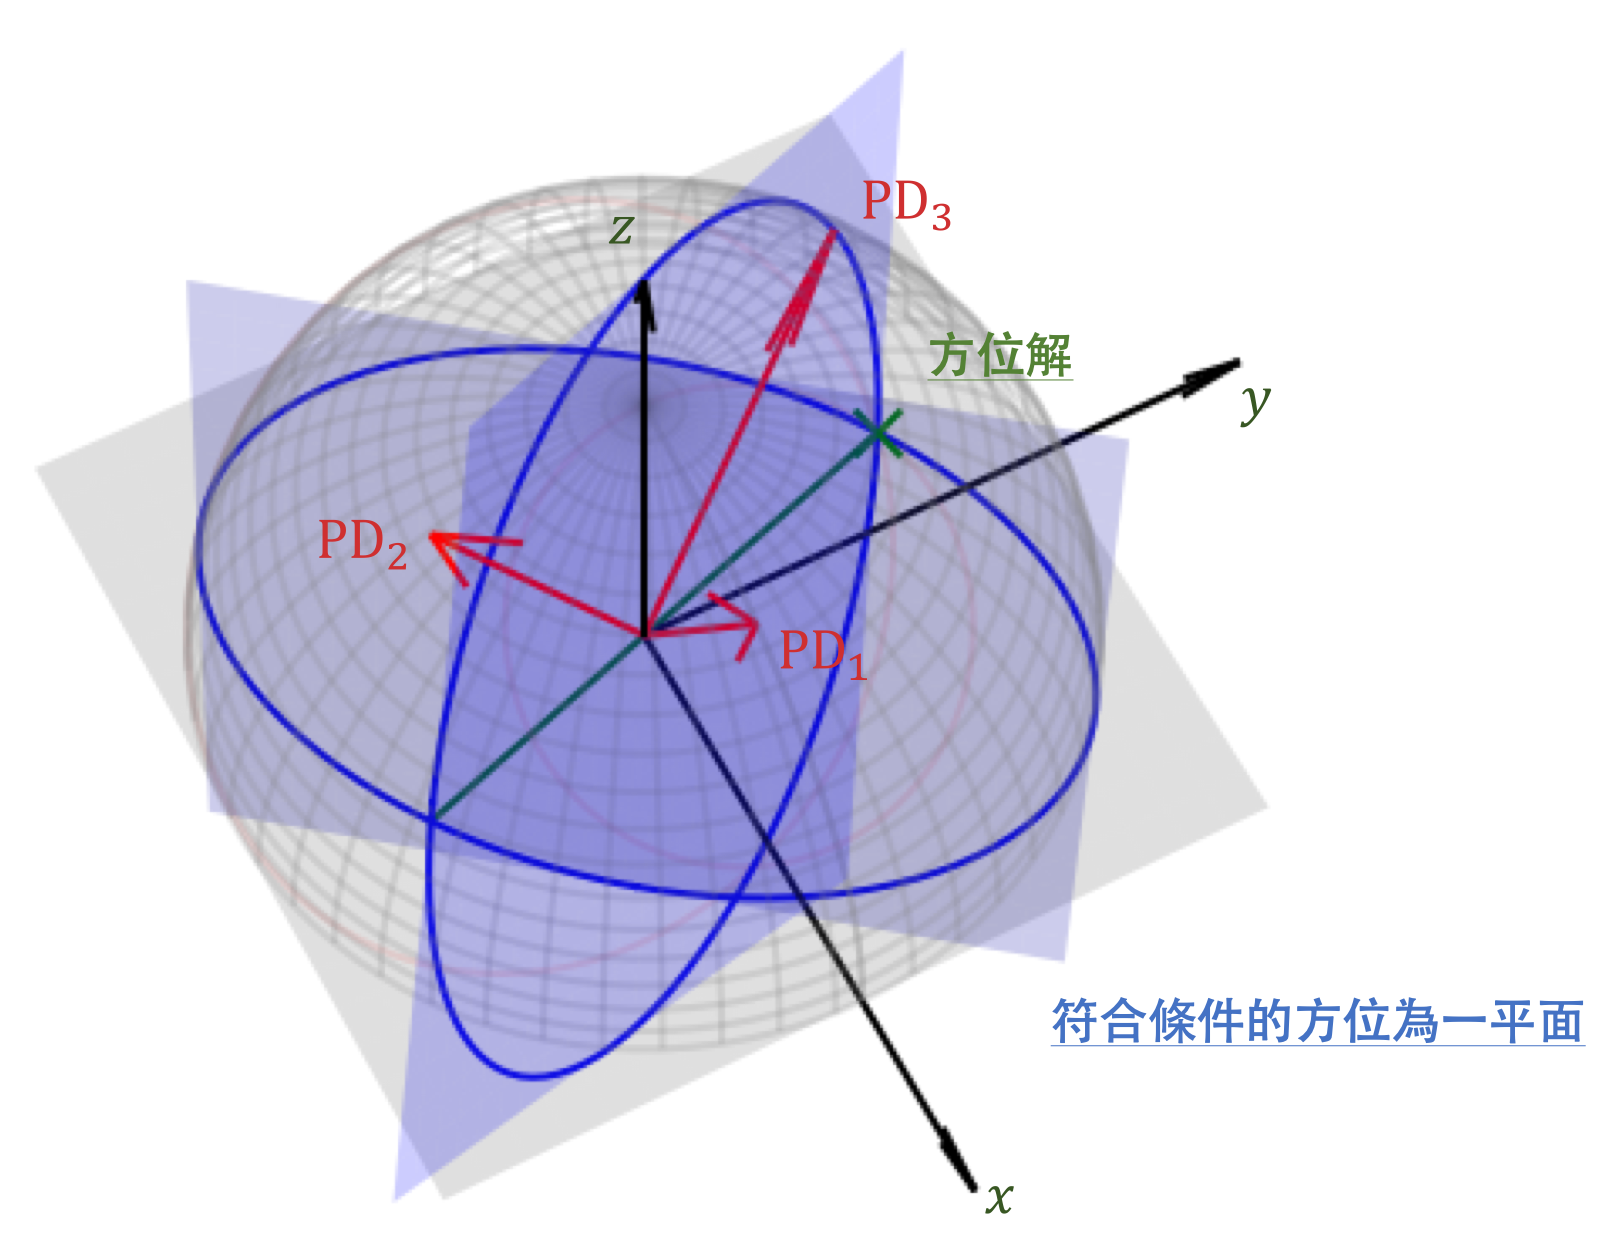
\includegraphics[width=9cm]{ch3pic/solve_axis.png}
            \caption{兩平面交於一軸}
            \label{pic:solve_axis}
        \end{figure}

        其中,兩平面交軸有正負兩個方向,我們可以透過PD可視範圍最大為$90^o$的特性,判斷出方位解為交軸的正方向還是負方向,呈現於式\ref{eqn:solve_axis}。
   
        \begin{gather}
            \label{eqn:solve_axis}
             \hat{{^{PL}\boldsymbol{Tv}}_{p{r_sr_c}}} = 
             \begin{cases}
                (\boldsymbol{N}_{pr_c}\times \boldsymbol{N}_{r_sr_c})&,(\boldsymbol{N}_{pr_c}\times \boldsymbol{N}_{r_sr_c})>0\\
                -(\boldsymbol{N}_{pr_c}\times \boldsymbol{N}_{r_sr_c})&,\text{else}
             \end{cases}
        \end{gather}

        在此步驟,我們利用\ref{chp:cosine_ratio}章中產生的$Fp_l-1$個平面,選擇其中一個作為參考平面,將他以外的$Fp_l-2$個平面與其參考平面外積,得到共$Fp_l-2$個計算出的方位$\hat{{^{PL}\boldsymbol{Tv}}_{p{r_sr_c}}}$。


    \subsubsection{平均方位}
    \label{chp:orient_average}

        第$l$個LED與PD的電流資訊,可以解出$Fp_l-2$個方位,因此\textbf{該LED過濾後的訊號最少需被3個PD感測到,才得以解出方位。}而我們將$Fp_l-2$個方位平均,得到第$l$個LED利用$Fp_l$個資訊求出的方位$\hat{{^{PL}\boldsymbol{Tv}}_{l}}$。
        \begin{equation}
            \label{eqn:average_orient_led}
            \hat{{^{PL}\boldsymbol{Tv}}_{l}} = \frac{\sum^{Fp_l-2}_{p=1}\hat{{^{PL}\boldsymbol{Tv}}_{p{r_sr_c}}}}{Fp_l-2}
        \end{equation}

        而一共有$l$個LED,我們再將$l$個LED獲得的方位$\hat{{^{PL}\boldsymbol{Tv}}_{l}}$平均,解出方位$\hat{{^{PL}\boldsymbol{Tv}}}$。

        \begin{equation}
            \label{eqn:average_orient}
            \hat{{^{PL}\boldsymbol{Tv}}} = \frac{\sum^{L}_{l=1}\hat{{^{PL}\boldsymbol{Tv}}_{l}}}{L}
        \end{equation}
        
        
    \subsubsection{小結}
    \label{chp:orient_conclu}

    計算方位的方法,是透過PD兩兩比較得到方位的可能平面解,再透過平面兩兩外積求交軸即為方位。然而由於$L$個LED與$P$個PD交互之下,兩兩比較便會變得很複雜,可以參考圖\ref{pic:algorithm_flow}中的流程較為清楚。在這之中,最少需要一個LED與三個訊號沒被過濾掉的PD訊號,才能夠解出方位。

        

         

    


    \subsection{求解距離}
    \label{chp:solve_D}

    在\ref{chp:solve_phi}章中解出方位後,對於光傳遞模型(式\ref{chp:model_mul})中的變數,我們目前僅能夠得到入射角$\phi_{lp}$的資訊,仍缺少出射角資訊以求距離。因此,求解距離的步驟可參考圖\ref{pic:algorithm_flow},需要先解出PD座標系於LED座標系上的方位,再利用方位資訊解出出入射角,進而利用光傳遞模型解出距離,以下分小節介紹。

        \subsubsection{解LED座標系中PD座標系所在方位}
        \label{chp:solve_theta}

        我們可以利用\ref{chp:solve_phi}章中一樣的方法,改應用在LED座標系中,解出PD座標系於LED座標系上的方位$\hat{{^{LP}\boldsymbol{Tv}}}$。方法與\ref{chp:solve_phi}章完全相同,以下僅簡單介紹:

        針對第$p$個PD的資訊,在訊號過濾後,總共接收到$Fl_p$個LED訊號。而由於硬體擺放位置皆限制於座標系原點,因此參考圖\ref{pic:mulled_1pd},式\ref{eqn:model_algorithm_filter}中的三個變數僅剩下LED出射角$\theta_{lp}$,即可透過兩兩比較,得到$Fl_p-1$個出射角餘弦比值,而滿足出射角餘弦比值的方位為通過原點的平面。
        
        \begin{figure}[h!]
            \centering
            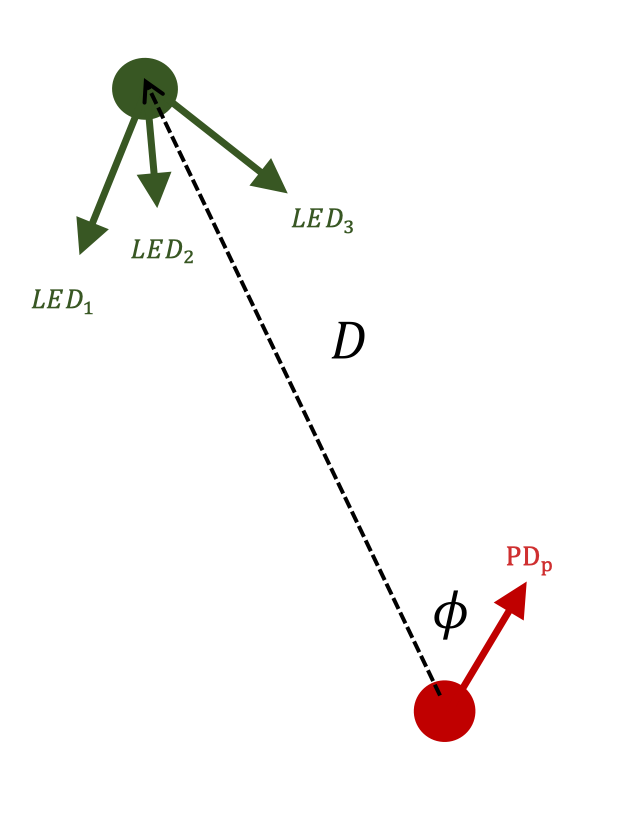
\includegraphics[width=6cm]{ch3pic/mulled_1pd.png}
            \caption{多LED對同一PD之間的幾何關係}
            \label{pic:mulled_1pd}
        \end{figure}

        再來,同樣取一平面作為參考,將其餘平面與參考平面外積,得到共$Fl_p-2$個方位$\hat{{^{LP}\boldsymbol{Tv}_{lr_sr_c}}}$(參考式\ref{eqn:solve_axis})。最後將第$p$個PD獲得的$Fl_p-2$個方位平均得$\hat{{^{LP}\boldsymbol{Tv}_{p}}}$,再將總共$P$個PD所得方位平均,即可獲得PD座標系於LED座標系上的方位$\hat{{^{LP}\boldsymbol{Tv}}}$,可以參考圖\ref{pic:algorithm_coor}。


        \subsubsection{解出LED與PD的出入射角}
        \label{chp:solve_ang}

        有了\ref{chp:solve_phi}章中求出的PD座標系中LED所在方位$\hat{{^{PL}\boldsymbol{Tv}}}$,我們利用PD硬體指向$^P\boldsymbol{V}_p$與方位的內積獲得各PD的入射角$\hat{\phi_{lp}}$,如式\ref{eqn:solve_inang}。
        
        \begin{equation}
            \label{eqn:solve_inang}
            \hat{\phi_{lp}} = \arccos(\hat{{^{PL}\boldsymbol{Tv}}}\cdot ^P\boldsymbol{V}_p)
        \end{equation}
        
        出射角則是利用\ref{chp:solve_theta}章中求出PD座標系於LED座標系的方位$\hat{{^{LP}\boldsymbol{Tv}}}$,同樣與LED指向內積,得到各LED的出射角$\hat{\theta_{lp}}$,如式\ref{eqn:solve_outang}。

        \begin{equation}
            \label{eqn:solve_outang}
            \hat{\theta_{lp}} = \arccos(\hat{{^{LP}\boldsymbol{Tv}}}\cdot ^L\boldsymbol{V}_l)
        \end{equation}

        \subsubsection{利用光傳遞模型取得距離並平均}
        \label{chp:dis_average}

        光傳遞模型中(式\ref{eqn:model_algorithm_filter}),三個變數中的出入射角$\theta\phi$,已於式\ref{eqn:solve_outang}與式\ref{eqn:solve_inang}中求得,因此可求出唯一未知的變數距離$D$,呈現於下式\ref{eqn:solve_dis}

        \begin{equation}
            \label{eqn:solve_dis}
            \begin{aligned}
            \hat{t_d },_{lp} &= \sqrt[2]{\frac{ReAPt (Ml_{l}+1)}{2\pi}
                \frac{\cos\phi_{lp}^{Mp_{p}}\cos \theta_{lp}^{Ml_{l}} }
                {Ie_{lp}}
            }\\
            & = \sqrt[2]
            {
                \frac{ReAPt (Ml_{l}+1)}{2\pi}
                \frac{
                    (\hat{{^{PL}\boldsymbol{Tv}}}\cdot ^P\boldsymbol{V}_p)^{Mp_{p}}
                    (\hat{{^{LP}\boldsymbol{Tv}}}\cdot ^L\boldsymbol{V}_l)^{Ml_{l}} }
                {Ie_{lp}}
            }
            \end{aligned}
        \end{equation}


        式\ref{eqn:solve_dis}中得到的$L\times P$個距離解,於式\ref{eqn:average_dis}中平均得到解。

        \begin{equation}
            \label{eqn:average_dis}
            \hat{t_d }= \frac{\sum^{L}_{l=1}\sum^{P}_{p=1} \hat{t_d },_{lp} }{L\times P}
        \end{equation}

        \subsubsection{小結}

        如\ref{chp:orient_conclu}章所述,最少需要一個LED與3個PD才能獲得方位$\hat{{^{PL}\boldsymbol{Tv}}}$;而概念相同,PD座標系於LED座標系中的方位$\hat{{^{LP}\boldsymbol{Tv}}}$,則需要至少一個PD與3個LED才能解,進而得到距離資訊。\textbf{綜合兩者,我們需要最少三個LED對三個PD才能同時得到LED與PD於對方座標系中的方位$\hat{{^{PL}\boldsymbol{Tv}}}$,進而解出距離$\hat{t_d}$。}綜合方位與距離,相對位置以卡氏座標系表示如式\ref{eqn:solu}


        \begin{equation}
            \label{eqn:sollu}
            \hat{^{PL}\boldsymbol{T} }= \hat{t_d} \times {^{PL}\boldsymbol{Tv}} 
        \end{equation}

\section{演算法優點與缺點}
\label{chp:algorithm_ad_dis}


介紹完本研究所提出的演算法,這裡以條列分析此演算法的優缺點:


\begin{description}
    \item[1. 優點:]\hfill
    
    \begin{description}
        \item[- 目標平面與量測平面不需平行:]\hfill
        
        \qquad
        現今研究中,單點對單點的LED與PD定位系統,大多會限制目標物需與量測者平行,此限制是為了使式\ref{eqn:model}光傳播模型中的出入射角相等$\phi=\theta$,進而降低模型複雜度。然而,限制兩平面平行會讓使用情境十分受限,僅能使用在兩相對旋轉並不會改變的物體上,在實務上並不常見,例如室內光源搭配地面平放的物體。而本章節提出的演算法突破此限制,因此在使用情境上不受限,得以對空間中任意姿態的兩物進行相對位置量測,例如姿態會改變的人、機械手臂、載具等,族繁不及備載。
    
        \item[- 考量LED與PD的朗博次方:]\hfill
        
        \qquad
        完整的考量LED與PD的朗博次方,可使挑選LED與PD的硬體時,更貼近實際的情況,讓購買硬體時選擇不用侷限在朗博次方為一的選項中,使系統的靈活度更高。

        \item[- 可獲得三維定位:] \hfill
        
        \qquad
        此演算法可獲得三維定位資訊,並不需要事先獲得垂直距離資訊,因此在使用場域上也更為靈活,不需限制活動範圍為特定距離之平面。

        \item[- 可獲得目標物姿態:] \hfill
        
        \qquad
        本研究提出的方法除了三維相對位置$^{PL}\boldsymbol{T}$,還能夠得到目標物的姿態,也就是LED座標系中PD座標系所在方位$^{LP}\boldsymbol{Tv}$,這項資訊在LED與PD定位方法中較少出現。
        
        \item[- 硬體配置靈活度較高:] \hfill
        
        \qquad
        此演算法中,對於LED與PD的指向並沒有特別的限制,不像大多文獻中常見將組態中的天頂角$\alpha$限制為相同;除此之外,LED與PD數量也可改變,只要兩者數量都大於三,可視範圍內便可進行定位。因此靈活度高,設計上可調整的變數多,即可針對不同情境調整。
    
    \end{description}

    \item[2. 缺點:] \hfill
    
    \begin{description}
        \item[- 演算法較為複雜:]  \hfill
        
        \qquad
        限制多的演算法,大多可以透過簡單的矩陣或方程式運算得到定位;相較起來,本研究所提出的演算法需要先解出兩座標系於對方座標系中的方位,進而計算出$L\times P$個出入射角來計算距離,演算法較為複雜。

        \item[- 多LED對多PD定位系統的難度:] \hfill
        
        \qquad
        多LED與多PD的定位系統,由於光通訊的硬體尚未被商業化,因此在文獻上較少有硬體的實驗驗整,所以在評估演算法時,大多僅能透過模擬。這樣會使評估缺乏可信度,無法討論多LED對多PD定位下的實務問題,僅能夠探討系統發展的可能性,而模擬與實際上的差異則需要被注意。
    \end{description}
    
\end{description}

介紹完本研究提出的演算法後,我們需要分析此演算法在定位上的效果,以及各參數對定位表現的影響,因此於第\ref{chp:4}章中,建立模擬環境模擬多LED與多PD的定位系統,套用本章節提出的定位演算法,進行誤差分析。










